\title{ALPSチュートリアル -- ALPSの概要}

\begin{document}

\lstset{language={C++},showspaces=false,rulecolor=\color[cmyk]{0, 0.29,0.84,0}}

\begin{frame}
  \titlepage
\end{frame}

\section*{Outline}
\begin{frame}
  \tableofcontents
\end{frame}

\section{チュートリアルの概要}

\begin{frame}
  \frametitle{ALPSチュートリアル 資料}
  \begin{itemize}
    \setlength{\itemsep}{1em}
  \item ALPSチュートリアル資料(日)
    \begin{itemize}
      \item PDF: {\footnotesize \url{http://sf.net/projects/alps-tutorial/files/}}
      \item \TeX ソース: {\footnotesize \url{https://github.com/cmsi/alps-tutorial/}}
    \end{itemize}
  \item ALPSオフィシャルページ(英日): {\footnotesize \url{http://alps.comp-phys.org/}}
  \item ALPS Developer Wiki (英): {\footnotesize \url{http://alps.comp-phys.org/trac/}}
  \item CMSI MateriApps: {\footnotesize \url{http://ma.cms-initiative.jp/}}
    \begin{itemize}
      \item ALPS web講習会: {\footnotesize \href{http://ma.cms-initiative.jp/ja/listapps/alps/ju6d5o/llgd83}{http://ma.cms-initiative.jp/jp/...}}
    \end{itemize}
  \item 藤堂眞治「``実験技術''としての量子多体系シミュレーションソフトウェアALPS」日本物理学会誌 (掲載予定)
  \end{itemize}
\end{frame}

\begin{frame}{困った時は…}
  \begin{itemize}
    \setlength{\itemsep}{1em}
  \item ALPSサポートチーム(日): {\footnotesize \href{mailto:alps@exa.phys.s.u-tokyo.ac.jp}{alps@exa.phys.s.u-tokyo.ac.jp}}
  \item MateriApps ALPS フォーラム(日):

    {\footnotesize \href{http://ma.cms-initiative.jp/ja/community/materiapps-messageboard/alps}{http://ma.cms-initiative.jp/ja/community/materiapps-...}}
  \item ALPS User's Mailing List (英):

    {\footnotesize \href{https://alps.comp-phys.org/mediawiki/index.php/Forum:Overview}{https://alps.comp-phys.org/mediawiki/index.php/Forum...}}
  \end{itemize}
\end{frame}

\begin{frame}{ALPSチュートリアル スタッフ}
  \begin{itemize}
  \item チュートリアル資料作成・講師
    \begin{itemize}
    \item 藤堂眞治 (東大院理/物性研)
    \item 松尾春彦 (RIST)
    \item 五十嵐亮 (東大物性研)
    \item 本山裕一 (東大物性研)
    \item 諏訪秀麿 (東大院理)
    \end{itemize}
  \item 主催
    \begin{itemize}
    \item CMSI: 計算物質科学イニシアティブ \url{http://cms-initiative.jp/}
    \end{itemize}
  \item 共催
    \begin{itemize}
    \item RIST: 一般財団法人 高度情報科学技術研究機構 \url{http://www.rist.or.jp/}
    \end{itemize}
  \end{itemize}
\end{frame}

\begin{frame}
  \frametitle{チュートリアルの流れ}
  \begin{tabular}{|l|l|c|c|c|}
        \hline
        ALPSの概要 & {\tt 01\_overview} & {\footnotesize\color{red} ○} & {\footnotesize\color{blue} ◎} & {\footnotesize\color{green} ◎} \\
        \hline
        ALPSのインストール & {\tt 02\_installation} & {\footnotesize\color{red} ◎} & {\footnotesize\color{blue} ◎} & {\footnotesize\color{green} ◎} \\
        \hline
        アプリケーション実習(1) & {\tt 03\_tutorial} & {\footnotesize\color{red} ◎} & {\footnotesize\color{blue} ◎} & {\footnotesize\color{green} ◎} \\
        \hline
        Python入門 & {\tt 04\_python} & {\footnotesize\color{red} ○} & {\footnotesize\color{blue} ○} & {\footnotesize\color{green} ◎} \\
        \hline
        ALPS Python入門 & {\tt 05\_pyalps} & {\footnotesize\color{red} ○} & {\footnotesize\color{blue} ○} & {\footnotesize\color{green} ◎} \\
        \hline
        Matplotlib入門 & {\tt 06\_matplotlib} & {\footnotesize\color{red} ○} & {\footnotesize\color{blue} ○} & {\footnotesize\color{green} ◎} \\
        \hline
        アプリケーション実習(2) & & {\footnotesize\color{red} ◎} & {\footnotesize\color{blue} } & {\footnotesize\color{green} ◎} \\
        \hline
        アプリケーションのALPS化 & {\tt 07\_alpsize} & {\footnotesize\color{red} } & {\footnotesize\color{blue} ◎} & {\footnotesize\color{green} ◎} \\
        \hline
  \end{tabular}
  
  {\footnotesize\color{red} ○}: ユーザコース, {\footnotesize\color{blue} ○}: 開発者コース {\footnotesize\color{green} ○}: 集中コース
\end{frame}

\begin{frame}
  \frametitle{ALPSチュートリアルの目標}
  \begin{itemize}
    \setlength{\itemsep}{1em}
    \item ALPSの概要を知る \ [{\footnotesize\color{red} ○}{\footnotesize\color{blue} ○}{\footnotesize\color{green} ○}]
    \item ALPSアプリケーションの実行方法を学ぶ  \ [{\footnotesize\color{red} ○}{\footnotesize\color{blue} ー}{\footnotesize\color{green} ○}]
    \item ALPS Pythonツールを使った結果の解析方法を学ぶ  \ [{\footnotesize\color{red} ○}{\footnotesize\color{blue} ー}{\footnotesize\color{green} ○}]
    \item ALPSライブラリの仕組みを学ぶ \ [{\footnotesize\color{red} ー}{\footnotesize\color{blue} ○}{\footnotesize\color{green} ○}]
    \item ユーザアプリケーションの作成方法を学ぶ  \ [{\footnotesize\color{red} ー}{\footnotesize\color{blue} ○}{\footnotesize\color{green} ○}]
    \item (ALPSチュートリアルの問題点を洗い出し改良する) \ [{\footnotesize\color{red} ◎}{\footnotesize\color{blue} ◎}{\footnotesize\color{green} ◎}] 
  \end{itemize}
\end{frame}

\section{量子格子模型とは?}
\subsection*{{\protect\color{red}●}{\protect\color{blue}●}}

\begin{frame}{量子格子模型: Quantum Lattice Models}
  \begin{columns}[T]
    \begin{column}{.8\textwidth}
      \begin{itemize}
      \item 量子スピン模型(XXZ模型) \begin{equation*} {\cal H} = \frac{J^{xy}}{2}
        \sum_{\langle i,j \rangle} (S^+_i S^-_j + S^-_i S^+_j) + J^z
        \sum_{\langle i,j \rangle} S^z_i S^z_j \end{equation*}
      \item Hubbard模型 \begin{equation*} {\cal H} = -t \sum_{\langle i,j \rangle \sigma}
        (c^\dagger_{i\sigma} c_{j\sigma} + \mbox{h.c.}) + U \sum_{i}
        n_{i\uparrow} n_{i\downarrow} \end{equation*}
      \item t-J模型 \begin{equation*} {\cal H} = -t \sum_{\langle i,j \rangle \sigma}
        (c^\dagger_{i\sigma} c_{j\sigma} + \mbox{h.c.}) + J \sum_{i,j}
        ({\bf S}_i \cdot {\bf S}_j - n_{i} n_{j} / 4) \end{equation*}
      \end{itemize}
    \end{column}
    \begin{column}{.2\textwidth}
      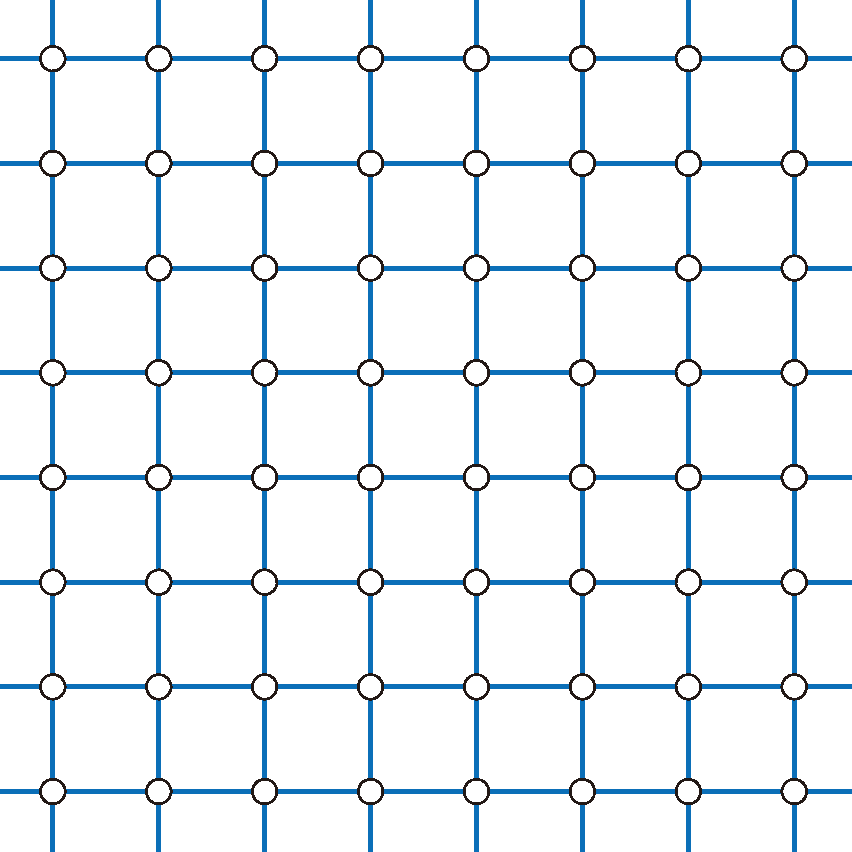
\includegraphics[width=\textwidth]{square.pdf}
    \end{column}
  \end{columns}
\end{frame}

\begin{frame}{なぜQLMを考えるのか?}
  \begin{columns}[T]
    \begin{column}{.2\textwidth}
      \includegraphics[width=\textwidth]{ising-tc.png} \\
      \includegraphics[width=\textwidth]{qcp.pdf}
    \end{column}
    \begin{column}{.8\textwidth}
      \begin{itemize}
        %\setlength{\itemsep}{1em}
      \item 量子多体系における強相関効果
        \begin{itemize}
        \item さまざまな秩序状態
        \item 量子的に強くゆらいだ相: 量子液体, スピンギャップ相
        \item 量子相転移, 量子臨界現象
        \end{itemize}
      \item 量子統計物理におけるユニバーサリティー
        \begin{itemize}
        \item 量子臨界現象は系の次元, 秩序変数の対称性などにしか依存しない
        \item 量子臨界現象特有のユニバーサリティークラスの探索
        \end{itemize}
      \item 新しい計算物理学的手法の発展
        \begin{itemize}
        \item 量子モンテカルロ法, DMRG, DMFT, テンソルネットワーク, など
        \end{itemize}
      \end{itemize}
    \end{column}
  \end{columns}
\end{frame}

%\begin{frame}{実験室で実現されているQLM}
%\end{frame}

%\begin{frame}{Finite-size scaling analysis}
%\end{frame}
  
\section{ALPSプロジェクト}
\subsection*{{\protect\color{red}●}{\protect\color{blue}●}}

\begin{frame}
  \frametitle{ALPSプロジェクトの目標}
  \begin{itemize}
    \setlength{\itemsep}{1em}
  \item 量子統計物理分野の現状
    \begin{itemize}
    \item 研究グループ毎に異なるコードを開発
    \item シミュレーションを行う模型毎に異なる実装
    \item アルゴリズムはますます複雑になりソフトウェア開発が長期化
    \item 可搬性・互換性のない入出力形式
    \end{itemize}
  \item ALPSプロジェクトの目標
    \begin{itemize}
    \item 最新のアルゴリズムを用いた``community code''の開発
    \item 大規模並列計算などのためのC++ライブラリ・フレームワーク開発
    \item 統一入出力形式の提案とそれにもとづくデータ解析ツールの作成
    \item 計算物理の専門家だけでなく, 理論家・実験家にも使えるシミュレーションソフトウェア
    \end{itemize}
  \end{itemize}
\end{frame}

\begin{frame}{ALPSとは?}
  ALPS = \alert{A}lgorithms and \alert{L}ibraries for \alert{P}hysics \alert{S}imulations
  %\begin{columns}[T]
    %\begin{column}{.7\textwidth}
      \begin{itemize}
      \item 量子スピン系, 電子系など強相関量子格子模型のシミュレーショ
        ンためのオープンソースソフトウェアの開発を目指す国際共同プロジェ
        クト
        %\begin{itemize}
        \item ALPSライブラリ = C++による格子模型のための汎用ライブラリ群
        \item ALPSアプリケーション = 最新のアルゴリズムに基づくアプリケーション群: QMC, DMRG, ED, DMFT等
        \item ALPSフレームワーク = 汎用入出力形式, 解析ツール, スケジュー
          ラなど, 大規模並列シミュレーションのための環境
        %\end{itemize}
      \end{itemize}
    %\end{column}
    %\begin{column}{.3\textwidth}
      %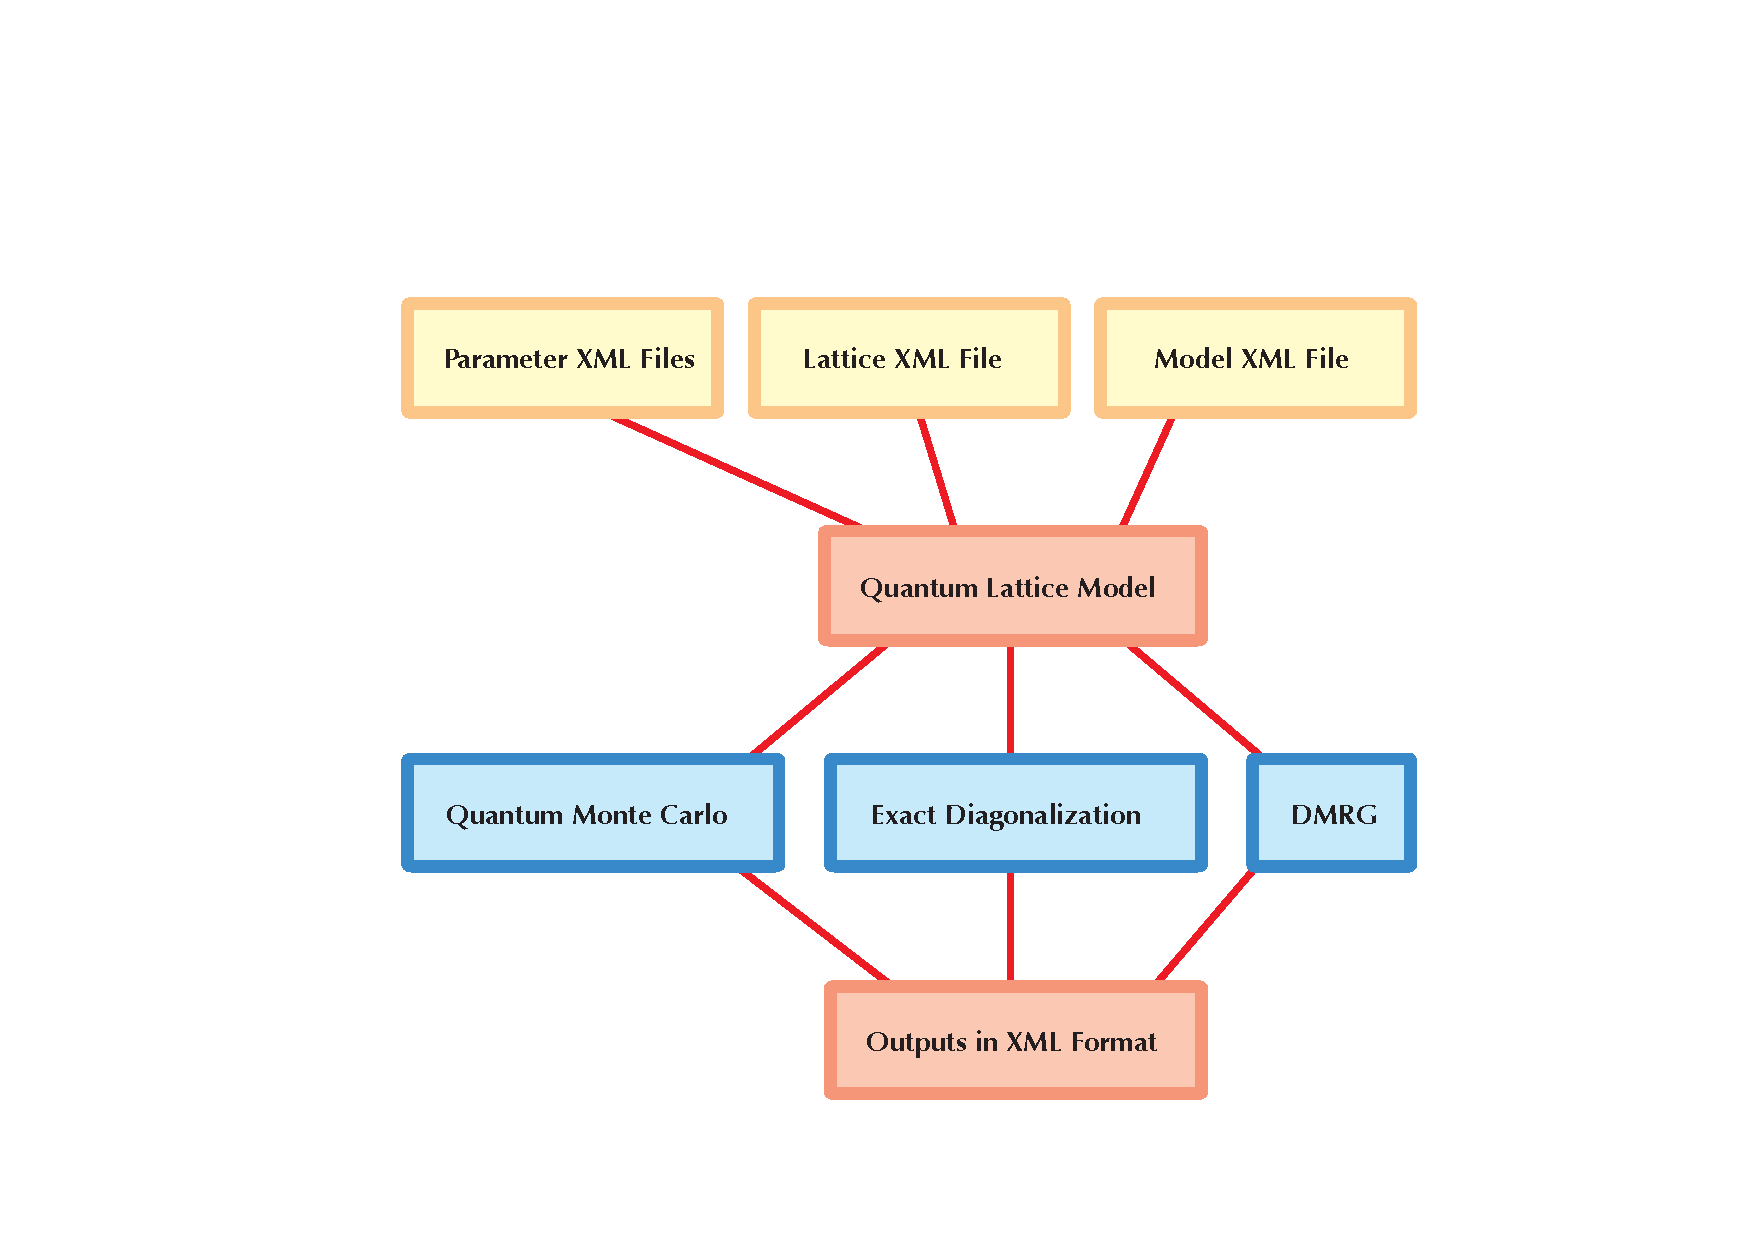
\includegraphics[width=1.2\textwidth]{simulation.pdf}
    %\end{column}
  %\end{columns}
\end{frame}

\begin{frame}{ターゲット・オーディエンス}
  \begin{itemize}
    \setlength{\itemsep}{1em}
  \item 実験家
    \begin{itemize}
    \item 物質のモデリングにソフトウェアパッケージを利用
    \item 実験結果とシミュレーション結果のフィッティングにより, 相互作用定数などを決定
    \end{itemize}
  \item 理論家
    \begin{itemize}
    \item 理論的なアイデアのチェックに使いやすい整備されたコードを利用
    \item 自前のコードのデバッグに
    \item 新しいコード開発の基盤としての利用
    \end{itemize}
  \item 計算機科学者, 学生, $\cdots$
  \end{itemize}
\end{frame}

\section{ALPSの開発}
\subsection*{{\protect\color{red}●}{\protect\color{blue}●}}

\begin{frame}
  \frametitle{基盤となる技術}
  \begin{itemize}
    \setlength{\itemsep}{1em}
  \item C++によるジェネリック・プログラミング
    \begin{itemize}
    \item C++標準テンプレートライブラリ
    \item Boost C++ ライブラリ \url{http://www.boost.org/}
    \item ALPS独自のクラス, ジェネリック・アルゴリズムを実装
    \item 柔軟性, 再利用性, 高信頼性, 高性能を同時に達成
    \end{itemize}
  \item XML, HDF5 \url{http://www.hdfgroup.org/HDF5/}による入出力
    \begin{itemize}
    \item 可搬性, 自己記述性, 変換が容易
    \end{itemize}
  \item 量子格子模型に対する最新のシミュレーション手法
  \end{itemize}
\end{frame}

\begin{frame}
  \frametitle{なぜC++を使うのか?}
  \begin{columns}[T]
    \begin{column}{.5\textwidth}
      \centering \includegraphics[width=4.5cm]{modern-cxx.pdf}
    \end{column}
    \begin{column}{.5\textwidth}
      \centering \includegraphics[width=4.5cm]{cxx-template.pdf}
    \end{column}
  \end{columns}
\end{frame}

\begin{frame}
  \frametitle{ALPSの歴史}
  \begin{itemize}
  \item 1990年代中頃 ALPSの前身となる PALM C++, DMRG, looper などが開発される
  \item 2002年 ALPSプロジェクト始動
  \item 2004年 バージョン1.0, 第1回 Users Workshop
  \item 2010年 バージョン2.0
  \item 2014年10月現在
    \begin{itemize}
      \item ソースコード: C++ 396,000行, Python 39,000行, Fortran 10,000行
      \item 開発者: 約30名(7ヶ国)
    \end{itemize}
  \end{itemize}
\end{frame}

\begin{frame}
  \frametitle{ALPSの開発者}
  \begin{columns}[T]
    \begin{column}{.34\textwidth}
      \begin{itemize}
      \item Austria
        \begin{itemize}
        \item H. G. Evertz
        \end{itemize}
      \item France
        \begin{itemize}
        \item O. Parcollet
        \end{itemize}
      \item Germany
        \begin{itemize}
        \item S. Fuchs
        \item G. Guertler
        \item D. Koop
        \item U. Schollw\"ock
        \item S. Trebst
        \item S. Wessel
        \end{itemize}
      \item Poland
        \begin{itemize}
        \item G. Pawlowski
        \end{itemize}
      \end{itemize}
    \end{column}
    \begin{column}{.34\textwidth}
      \begin{itemize}
      \item Switerland
        \begin{itemize}
        \item B. Bauer
        \item L. Gamper
        \item J. Gukelberger
        \item A. Hehn
        \item S. V. Isakov
        \item P. N. Ma
        \item P. Mates
        \item J. D. Picon
        \item L. Pollet
        \item B. Surer
        \item M. Troyer
        \item P. Werner
        \end{itemize}
      \end{itemize}
    \end{column}
    \begin{column}{.35\textwidth}
      \begin{itemize}
      \item Japan
        \begin{itemize}
        \item 五十嵐 亮
        \item 松尾春彦
        \item 藤堂眞治
        \end{itemize}
      \item USA
        \begin{itemize}
        \item L. D. Carr
        \item A. Feiguin
        \item J. Freire
        \item E. Gull
        \item E. Santos
        \item V. W. Scarlola
        \item C. Silva
        \item M. L. Wall
        \end{itemize}
      \end{itemize}
    \end{column}
  \end{columns}
\end{frame}

\subsection*{{\protect\color{red}ー}{\protect\color{blue}●}}

\begin{frame}
  \frametitle{開発のためのインフラストラクチャ}
  \begin{itemize}
  \item ソースコードの規模, 開発体制が大きくなると今までの方法では破綻する
  \item 開発・サポートのためのツールを一から作りあげるのは非現実的
  \item フリーソフトウェアの利用
    \begin{itemize}
    \item ビルドシステム: CMake
    \item ソースコードの管理: Subversion
    \item プロジェクト管理・バグ追跡: Trac
    \item ドキュメント作成: MediaWiki
    \item メーリングリスト: Mailman
    \end{itemize}
  \item Linux ワークステーションが1台あれば, これらの環境を整えるのは現在では比較的容易
  \end{itemize}
\end{frame}

\begin{frame}
  \frametitle{ビルドシステム: CMake}
  \begin{itemize}
    \setlength{\itemsep}{1em}
  \item Makefileを生成するためのユーティリティー (configureスクリプトに対応)
    \begin{itemize}
    \item Windows の Visual C++ 用ソリューションファイル, Mac OS X の Xcode 用プロジェクトファイルの生成も可能
    \end{itemize}
  \item 設定は CMakeLists.txt に記述する
  \item テスト(CTest)やバイナリ配布(CPack)の機能もある
  \item ファイルの依存関係の自動検出
  \end{itemize}
\end{frame}

\begin{frame}
  \frametitle{VCS (Version Control System)によるソース管理: Subversion}
  \begin{itemize}
  \item 開発者が複数になると, ディレクトリ名やログファイルによるバージョン管理はすぐに破綻する
  \item ソースコードをサーバー上で一括管理
    \begin{itemize}
    \item ネットワーク経由でソースを check out/check in
    \end{itemize}
  \item 更新毎に一意なバージョン番号を付与
  \item 全ての修正履歴を保存
  \item 複数人が同時に更新した場合に衝突を回避するしくみ
  \item ブランチ・マージ・タグ付けなどが可能
  \item 開発者が一人, 公開の予定がない場合でも積極的に使うべき
  \end{itemize}
\end{frame}

\begin{frame}
  \frametitle{BTS (Bug Tracking System) の利用: Trac}
  \begin{itemize}
    \setlength{\itemsep}{1em}
  \item プロジェクト管理とバグ追跡のためのツール
  \item Web ブラウザからアクセス・操作
    \begin{itemize}
    \item 開発者の情報共有のための wiki
    \item Subversion との連携 (ソース, 修正履歴の web 上での閲覧)
    \item プロジェクト管理 (ロードマップ, マイルストーンの管理)
    \item チケットシステム: バグやタスクの登録, 担当者の決定, 修正状況の追跡
    \end{itemize}
  \end{itemize}
\end{frame}

\begin{frame}
  \frametitle{Wikiによるマニュアル作成: MediaWiki}
  \begin{itemize}
  \item もともとはウィキペディアのために開発された
  \item Wiki とは?
    \begin{itemize}
    \item Webブラウザを利用してWeb文書を書き換えるシステム
    \item ネットワーク上のどこからでも書き換えができる
    \item 共同作業が容易
    \item Webブラウザがあれば編集作業が行える
    \item HTMLよりも簡潔な書式
    \item 文書間のリンクの作成が容易
    \end{itemize}
  \item ALPS Wiki のコンテンツ
    \begin{itemize}
    \item ニュース, インストール方法, ALPSに関連する論文, 発表資料, ライブラリリファレンスマニュアル, チュートリアル
    \end{itemize}
  \end{itemize}
\end{frame}

\begin{frame}
  \frametitle{メーリングリストの活用: Mailman}
  \begin{itemize}
    \setlength{\itemsep}{1em}
  \item 開発者メーリングリスト
    \begin{itemize}
    \item 開発方針に関する意見交換, リリーススケジュール調整, 担当者調整等
    \item Trac チケットの変更ログも自動的にここに流れる
    \end{itemize}
  \item ユーザメーリングリスト
    \begin{itemize}
    \item Web からの自動登録
    \item 開発者 + ユーザコミュニティーによるサポートの場
    \item FAQ ⇒ Wiki ドキュメントへ反映
    \item バグレポート, 要望など ⇒ Trac チケットへ
    \end{itemize}
  \end{itemize}
\end{frame}

\subsection*{{\protect\color{red}●}{\protect\color{blue}●}}

\begin{frame}
  \frametitle{ワークショップ}
  \begin{itemize}
    \setlength{\itemsep}{1em}
  \item ALPS developers workshop
    \begin{itemize}
      \item 今後の開発方針についてブレインストーミング・ディスカッション
      \item 年1回程度
    \end{itemize}
  \item ALPS users workshop / tutorial
    \begin{itemize}
      \item アルゴリズムについてのレビュートーク
      \item Wiki のチュートリアルを用いて ALPS の実習
      \item CMSI神戸ハンズオン: 3ヶ月毎にALPSチュートリアルを開催予定
    \end{itemize}
  \end{itemize}
\end{frame}

\begin{frame}
  \frametitle{ALPSの展開}
  \begin{itemize}
    \setlength{\itemsep}{1em}
  \item 上方展開 (大規模化・高性能化・並列化)
    \begin{itemize}
    \item 量子モンテカルロ法(ALPS/looper)の超並列化
    \item 高並列スケジューラ(ALPS/parapack)のハイブリッド多重並列化
    \item Fortran, C プログラムのための API 作成
    \end{itemize}
  \item 下方展開 (裾野を広げる)
    \begin{itemize}
    \item 実験家・理論家による幅広い利用の促進
    \item Windows/Macintosh 用バイナリインストーラの開発
    \item ワークフロー・履歴管理システムとの統合
    \item GUI (グラフィカルユーザインターフェース)の開発
    \end{itemize}
  \end{itemize}
\end{frame}

\begin{frame}
\frametitle{ALPS``cite-me''ライセンス}
%\begin{itemize}
%\item ALPS Library License, ALPS Application License
  \begin{itemize}
  \item GNU General Public License 2 (GPL2) を基本としたライセンス
  \item Non-commercial academic use の場合自由に利用可能
  \item 自由に再配布可
  \item ユーザが変更を施したコードも同じライセンスの下で再配布可
  \item ALPSを用いた研究成果を公表する場合には acknowledgement と論文の引用が義務 (ALPSをユーザーコードのテストのみに使った場合を含む)
    \begin{minipage}{.9\textwidth}
    \begin{block}{}
      1. In any scientific publication based wholly or in part on the
      Library, the use of the Library must be acknowledged and the
      publications listed in the accompanying CITATIONS.txt document
      must be cited.
    \end{block}
    \end{minipage}
  \end{itemize}
%\end{itemize}
\end{frame}

\begin{frame}
  \frametitle{参考文献}
  \begin{itemize}
  \item ALPS papers
    \begin{itemize}
    \item F. Alet et al. {\it The ALPS Project: Open Source Software for
      Strongly Correlated Systems}, \href{http://jpsj.ipap.jp/link?JPSJS/74S/30}{J. Phys. Soc. Jpn. Suppl. 74, 30 (2005)}.
    \item A.~F. Albuquerque et al. {\it The ALPS project release 1.3: open source software for strongly correlated systems}, \href{http://dx.doi.org/10.1016/j.jmmm.2006.10.304}{J. Mag. Mag. Mat. 310, 1187 (2007)}.
    \item B. Bauer et al. {\it The ALPS project release 2.0: Open source software for strongly correlated systems}, \href{http://iopscience.iop.org/1742-5468/2011/05/P05001}{J. Stat. Mech., P05001 (2011)}.
    \end{itemize}
  \end{itemize}
\end{frame}

\section{ALPSの構成}
\subsection*{{\protect\color{red}●}{\protect\color{blue}●}}

\begin{frame}{ALPSの階層構造}
  \begin{center}
    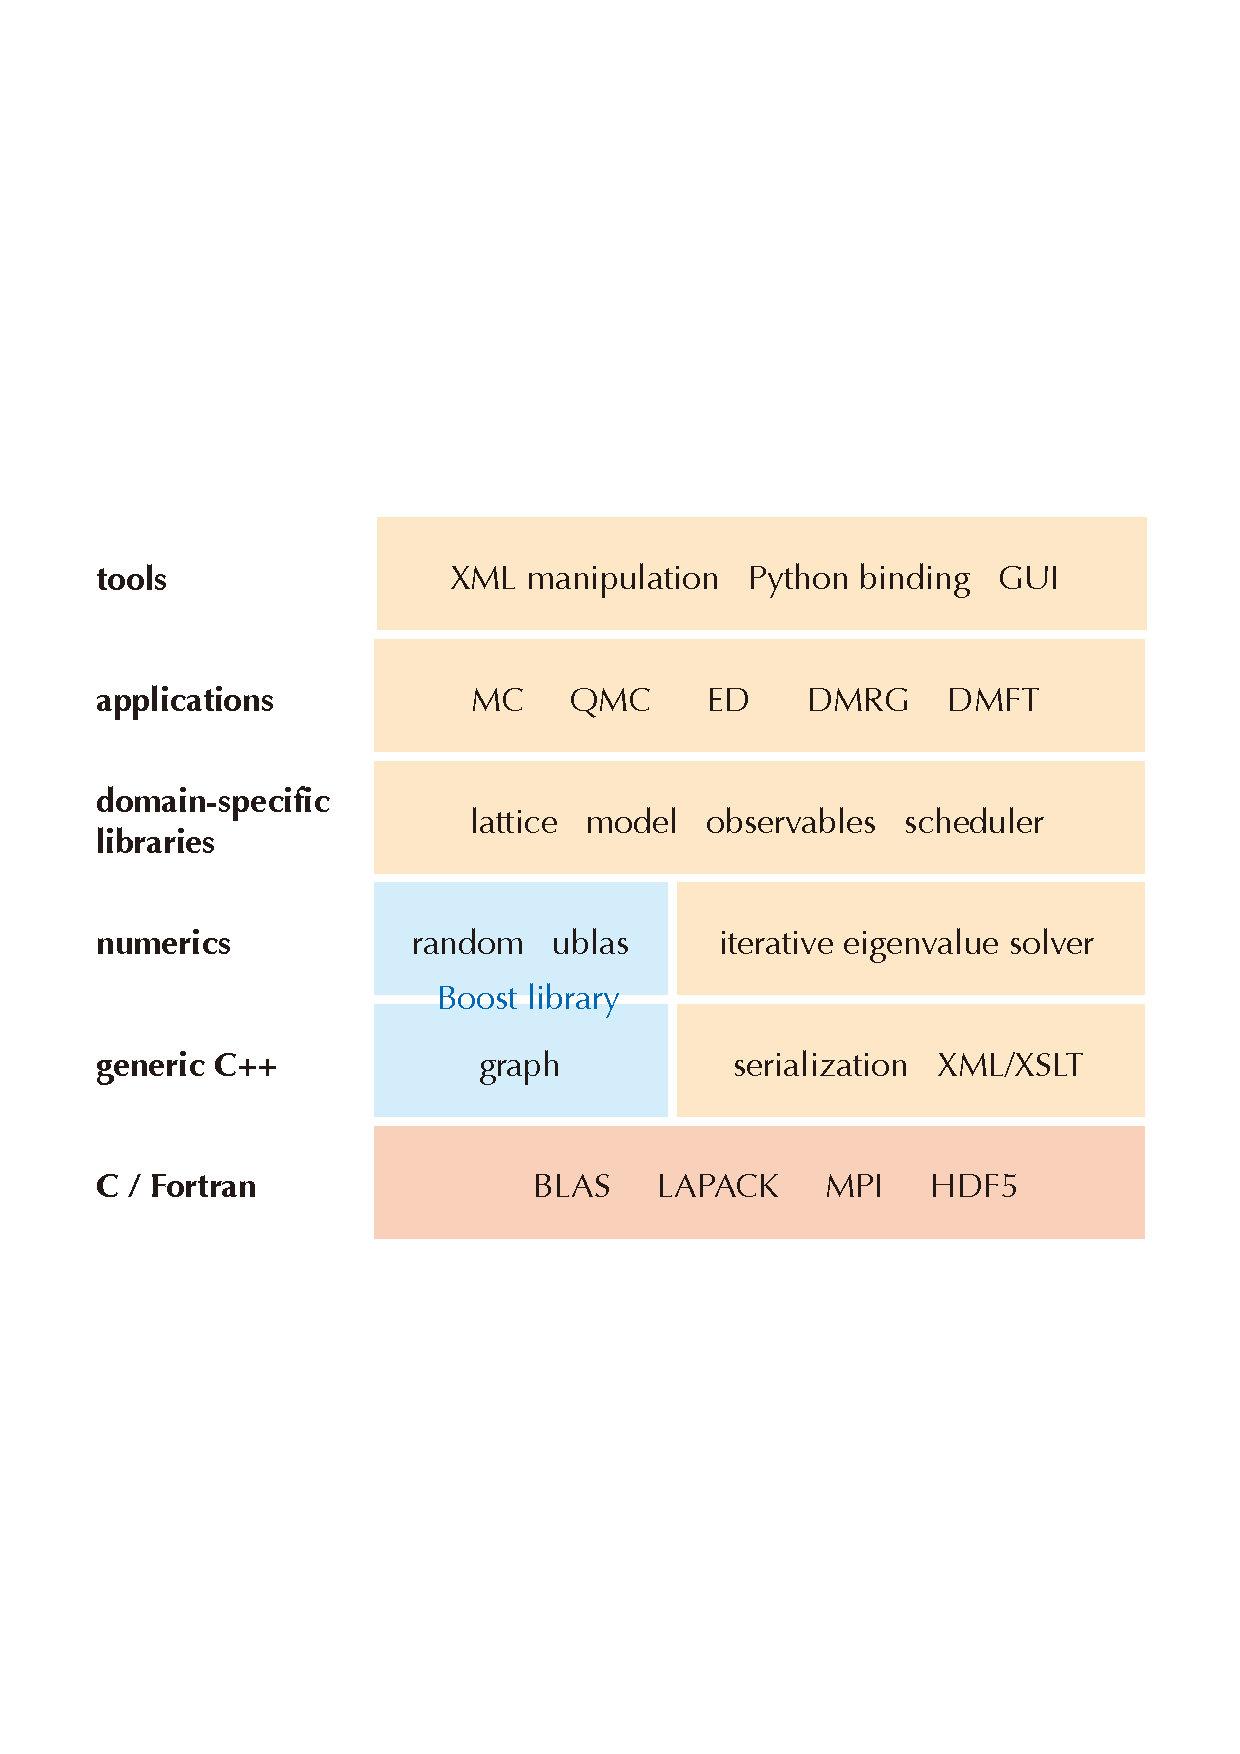
\includegraphics[height=0.65\textheight]{hierarchy.pdf}
  \end{center}
\end{frame}

\begin{frame}
  \frametitle{サードパーティーのライブラリ}
  \begin{itemize}
    \setlength{\itemsep}{1em}
  \item \href{http://www.netlib.org/blas/}{BLAS}, \href{http://www.netlib.org/lapack/}{LAPACK}: 線形演算(行列対角化, 特異値分解など) (オプション)
  \item \href{http://www.mpi-forum.org/}{MPI} (Message Passing Interface): 並列計算のためのメッセージ通信 (オプション)
  \item \href{http://www.hdfgroup.org/HDF5/}{HDF5} (Hierarchical Data Format): プラットフォーム非依存のバイナリファイル格納形式
  \item \href{http://www.boost.org/}{Boost C++ Library}: 乱数, グラフ, シリアル化, など多くの有用なライブラリ群
  \end{itemize}
\end{frame}

\section{ALPSライブラリ}
\subsection*{{\protect\color{red}●}{\protect\color{blue}●}}

\begin{frame}[t,fragile]
  \frametitle{ALPS/parameterライブラリ}
  \begin{columns}[T]
    \begin{column}{.5\textwidth}
      \begin{itemize}
      \item パラメータの入出力のためのライブラリ
        %\begin{itemize}
        \item 改行, セミコロン, コンマで変数を区別
        \item 四則演算, 初等関数(sin, cos, expなど)が使える
        \item $\pi$ (PI), 虚数単位(I)
          \item C 風, C++風のコメント
          \item \{ \} で囲まない変数は共通パラメータ
          \item \{ \} で囲んだ変数は異なるパラメータセット
        %\end{itemize}
      \end{itemize}
    \end{column}
    \begin{column}{.5\textwidth}
    \begin{lstlisting}
LATTICE = "chain lattice";
L = 16,
SEED = 2873
// C++ style comment
SWEEPS = 4096;
THERMALIZATION = SWEEPS/8;
/* C style comment */
{ T = 2; Sq = 2*PI/3; }
{ T = 1.8; }
\end{lstlisting}
    \end{column}
  \end{columns}
\end{frame}

\subsection*{{\protect\color{red}ー}{\protect\color{blue}●}}

\begin{frame}[t,fragile]
  \frametitle{ALPS/parameterを使ったコード例}
  \lstset{language={C++}}
  \begin{lstlisting}
#include <boost/foreach.hpp>
#include <alps/parameter.h>
int main() {
  std::ifstream fin;
  fin.open("parameters.txt");
  alps::ParameterList plist(fin);
  BOOST_FOREACH(alps::Parameters& p, plist) {
    double a = p["a"];
    double b = p.value_or_default("b", 0.5);
    ...
  }
  ...
}
\end{lstlisting}
\end{frame}

\subsection*{{\protect\color{red}●}{\protect\color{blue}●}}

\begin{frame}[t,fragile]
  \frametitle{ALPS/aleaライブラリ}
  \begin{itemize}
  \item マルコフ連鎖における平均値, 分散, 自己相関を計算するライブラリ
    \lstset{language={C++}}
    \begin{lstlisting}
alps::RealObservable mag2("Magnetization^2");
...
mag2 << m * m; // in each MC step
\end{lstlisting}
  \item ビンニング解析を用いた平均値, エラー, 自己相関時間の評価
    \lstset{language={C++}}
    \begin{lstlisting}
std::cout << mag2 << std::endl;
\end{lstlisting}
  \begin{itemize}
  \item 出力
\lstset{language={bash}}
\begin{lstlisting}
Magnetization^2: 1.5 +/- 0.707; tau = inf WARNING: check error convergence
\end{lstlisting}
  \end{itemize}
  \end{itemize}
\end{frame}

\subsection*{{\protect\color{red}ー}{\protect\color{blue}●}}

\begin{frame}[t,fragile]
  \frametitle{ALPS/aleaライブラリ}
  \begin{itemize}
  \item ジャックナイフ法を用いた非線形量のエラー評価
    \lstset{language={C++}}
    \begin{lstlisting}
alps::RealObsevaluator mag2eval(mag2);
alps::RealObsevaluator mag4eval(mag4);
alps::RealObsevaluator binder = mag2eval * mag2eval / mag4eval;
std::cout << binder;
\end{lstlisting}
  \begin{itemize}
  \item 出力
\lstset{language={bash}}
\begin{lstlisting}
(Magnetization^2) * (Magnetization^2) / (Magnetization^4): 0.45 +/- 0.25 WARNING: check error convergence
\end{lstlisting}
  \end{itemize}
  \end{itemize}
\end{frame}

\subsection*{{\protect\color{red}●}{\protect\color{blue}●}}

\begin{frame} [t,fragile,shrink]
  \frametitle{ALPS/latticeライブラリ}
  \begin{itemize}
    \setlength{\itemsep}{1em}
  \item 「格子構造」は数学的には「グラフ」で表現できる
    \begin{itemize}
    \item site $\Leftrightarrow$ vertex
    \item bond $\Leftrightarrow$ edge
    \end{itemize}
  \item Boost Graph Library に対する「ラッパー」を提供
    \begin{itemize}
    \item XMLによる「格子構造」の入出力
    \item 「ユニットセル」による繰り返し構造の指定
    \item 座標, パリティ, 逆格子ベクトルなどの属性
    \end{itemize}
  \item あらかじめ用意されている格子: "chain lattice", "square lattice", "triangular lattice", "honeycomb lattice", "simple cubic lattice", など
  \item ``printgraph'' で格子のチェック
  \end{itemize}
\end{frame}

\begin{frame}[t,fragile]
  \frametitle{有限格子 + ユニットセルの埋め込み - 1}
  \begin{itemize}
  \item 格子の指定
  \begin{lstlisting}
<LATTICE name="2D" dimension="2">
  <BASIS>
    <VECTOR>   1 0 </VECTOR>
    <VECTOR> 0.5 1 </VECTOR>
  </BASIS>
</LATTICE>
\end{lstlisting}
  \end{itemize}
  \begin{center}
    \includegraphics[height=0.3\textheight]{TutorialLatticeHOWTOLattice1}
  \end{center}
\end{frame}

\begin{frame}[t, fragile]
  \frametitle{有限格子 + ユニットセルの埋め込み - 2}
  \begin{itemize}
  \item ユニットセル
  \begin{lstlisting}
<UNITCELL name="simple1d" dimension="1" vertices="1">
  <EDGE>
    <SOURCE vertex="1" offset="0"/><TARGET vertex="1" offset="1"/>
  </EDGE>
</UNITCELL>
\end{lstlisting}
  \end{itemize}
  \begin{center}
    \includegraphics[height=0.25\textheight]{TutorialLatticeHOWTOLatticegraph3}
  \end{center}
\end{frame}

\begin{frame}[t,fragile]
  \frametitle{有限格子 + ユニットセルの埋め込み - 3}
  \begin{itemize}
  \item サイズ, 境界条件の指定
    \begin{lstlisting}
<LATTICEGRAPH name = "chain lattice">
  <FINITELATTICE>
    <LATTICE ref="chain lattice"/>
    <PARAMETER name="L"/>
    <EXTENT size ="L"/>
    <BOUNDARY type="periodic"/>
  </FINITELATTICE>
  <UNITCELL ref="simple1d"/>
</LATTICEGRAPH>
\end{lstlisting}
  \item より複雑な格子の作り方
    \begin{itemize}
    \item ALPS Lattice HOWTO: {\small \href{http://alps.comp-phys.org/mediawiki/index.php/Tutorials:LatticeHOWTO/ja}{http://alps.comp-phys.org/mediawiki/ index.php/Tutorials:LatticeHOWTO/ja}}
    \end{itemize}
  \end{itemize}
\end{frame}

\subsection*{{\protect\color{red}●}{\protect\color{blue}●}}

\begin{frame}[t,fragile]
  \frametitle{ALPS/modelライブラリ}
  \begin{itemize}
%    \setlength{\itemsep}{1em}
  \item XMLを使ってハミルトニアンを定義する
    \begin{itemize}  
    \item 量子数や演算子の定義
    \item シンボリックな表現を使って, ハミルトニアンのサイト項やボンド項を定義
    \end{itemize}
    \begin{lstlisting}
Jz*Sz(i)*Sz(j)+Jxy/2*(Splus(i)*Sminus(j)+Sminus(i)*Splus(j))
\end{lstlisting}
  \item 作成した局所ハミルトニアンは行列の形で取り出せる
  \item プラケット項などの多体相互作用は未対応
  \item ALPS Model HOWTO: {\small \href{http://alps.comp-phys.org/mediawiki/index.php/Tutorials:ModelHOWTO/ja}{http://alps.comp-phys.org/mediawiki/ index.php/Tutorials:ModelHOWTO/ja}}
  \item あらかじめ用意されている模型: "spin", "boson Hubbard", "hardcore boson", "fermion Hubbard", "alternative fermion Hubbard", "spinless fermions", "Kondo lattice", "t-J"
  \end{itemize}
\end{frame}

% \section{ALPS/scheduler}

% \section{HDF5とは?}

\section{ALPSアプリケーション}
\subsection*{{\protect\color{red}●}{\protect\color{blue}●}}

\begin{frame}
  \frametitle{ALPSアプリケーション}
  \begin{description}
  \item[fulldiag] {\color{red} 厳密対角化(全対角化法)}
  \item[sparsediag] {\color{red} 厳密対角化(Lanczos法)}
  \item[spinmc] 古典モンテカルロ法
  \item[loop] {\color{red} 量子モンテカルロ法(ループアルゴリズム)}
  \item[dirloop\_sse] {\color{red} 量子モンテカルロ(向き付きループアルゴリズム)}
  \item[worm] 量子モンテカルロ(ワームアルゴリズム)
  \item[dmrg,tebd] 密度行列繰り込み群
  \item[hirshfye,interaction,hybridization] 動的平均場近似のQMCソルバ
  \end{description}
\end{frame}

\begin{frame}
  \frametitle{厳密対角化}
  \begin{description}
  \item[fulldiag] 厳密対角化(全対角化法)
    \begin{itemize}
    \item ハウスホルダー法を用いて量子格子模型の全てのエネルギー固有値と固有状態を計算
    \item 任意の温度における物理量を数値誤差の範囲で厳密に計算
    \end{itemize}
  \item[sparsediag] 厳密対角化(Lanczos法)
    \begin{itemize}
    \item ランチョス法を用いて, 基底状態と少数の低励起状態を求める
    \end{itemize}
  \end{description}
  \begin{itemize}
  \item 全磁化などの保存量や系の並進対称性などを利用して, ヒルベルト空間の次元を削減
  \item 任意の局所的な演算子の期待値, 対角および非対角演算子の相関関数, 構造因子などの測定が可能
  \item 並列固有値ソルバライブラリRokkoと, それに基づく並列厳密対角化パッケージALPS/Baristaを開発中
  \end{itemize}
\end{frame}

\begin{frame}
  \frametitle{古典モンテカルロ法}
  \begin{description}
  \item[spinmc] 古典モンテカルロ法
    \begin{itemize}
      \item メトロポリス法あるいはクラスターアルゴリズム
      \item 古典スピン模型のモンテカルロシミュレーション
      \item 磁場中のイジング模型, XY模型, ハイゼンベルグ模型, ポッツ模型
    \end{itemize}
  \end{description}
\end{frame}

\begin{frame}
  \frametitle{量子モンテカルロ法}
  \begin{description}
  \item[loop] 量子モンテカルロ法(ループアルゴリズム)
    \begin{itemize}
      \item 連続虚時間ループアルゴリズム
      \item 時間反転対称性を持つ系(零磁場の場合、横磁場イジング模型など)に有効
      \item 2点相関関数(グリーン関数を含む)の計算
    \end{itemize}
  \item[dirloop\_sse] 量子モンテカルロ(向き付きループアルゴリズム)
    \begin{itemize}
      \item SSE (Stochastic Series Expansion)表示
      \item 磁場中スピン模型, ボーズハバード模型などに有効
    \end{itemize}
  \item[worm] 量子モンテカルロ(ワームアルゴリズム)
    \begin{itemize}
      \item 連続虚時間表示ワームアルゴリズム
      \item 非常に強い磁場が存在する場合などに有効
    \end{itemize}
  \end{description}
\end{frame}

\begin{frame}
  \frametitle{密度行列繰り込み群・動的平均場}
  \begin{description}
  \item[dmrg,tebd] 密度行列繰り込み群
    \begin{itemize}
      \item 一次元系・擬一次元系の基底状態および低励起状態を計算
      \item 局所的な物理量や2点相関関数の測定
      \item エンタングルメントエントロピーの測定
    \end{itemize}
  \item[hirshfye,interaction,hybridization] 動的平均場近似のQMCソルバ
    \begin{itemize}
      \item 系の自己エネルギーの波数依存性を無視することで, 多体フェルミオン模型を不純物問題に帰着
      \item Hirsch-Fye法{\tt hirshfye}
      \item 相互作用展開{\tt interaction}
      \item 混成状態展開{\tt hybridization}
    \end{itemize}
  \end{description}
\end{frame}

\begin{frame}{ALPSによるシミュレーション --- ワークフロー}
  \begin{center}
    \includegraphics[height=0.8\textheight]{workflow.pdf}
  \end{center}
\end{frame}

\end{document}
